
\documentclass[xcolor=dvipsnames]{beamer}  % for hardcopy add 'trans'

\mode<presentation>
{
  \usetheme{Singapore}
  % or ...
  \setbeamercovered{transparent}
  % or whatever (possibly just delete it)
}

\usefonttheme{professionalfonts}
\usepackage[russian]{babel}
% or whatever
%\usepackage[latin1]{inputenc}
% or whatever
%\usepackage{times}
%\usepackage[T1]{fontenc}
% Or whatever. Note that the encoding and the font should match. If T1
% does not look nice, try deleting the line with the fontenc.

%%%%%%%%%%%%%%%%%%%%%% start my preamble %%%%%%%%%%%%%%%%%%%%%%


\addtobeamertemplate{navigation symbols}{}{%
    \usebeamerfont{footline}%
    \usebeamercolor[fg]{footline}%
    \hspace{1em}%
    \insertframenumber/\inserttotalframenumber
} 

\setbeamercolor{footline}{fg=blue}
\setbeamerfont{footline}{series=\bfseries}


%\usepackage{epsfig}
\usepackage{graphicx}
\graphicspath{{./figs_code/}}

\usepackage{amsmath, amssymb, amsthm}

\usepackage{fancyvrb}

\usepackage{tikz}
\usetikzlibrary{arrows}
\usetikzlibrary{calc}
\usetikzlibrary{intersections}
\usetikzlibrary{decorations}
\usepackage{pgf}
\usepackage{pgfplots}
\pgfplotsset{compat=1.13}

\usepackage{graphviz}
 
\usepackage{verbatim}


\usepackage{algorithmicx,algpseudocode}


%font
\usepackage{mathpazo}
%\usepackage[usenames, dvipsnames]{color}

%\usepackage[linesnumbered, ruled, lined]{algorithm2e}

\usepackage{xr}
\externaldocument[ET-]{et}


\newcommand*{\theorembreak}{\usebeamertemplate{theorem end}\framebreak\usebeamertemplate{theorem begin}}

\newcommand{\newtopic}[1]{\textcolor{Green}{\Large \bf #1}}
\newcommand{\navy}[1]{\textcolor{Blue}{\bf #1}}
\newcommand{\navymth}[1]{\textcolor{Blue}{#1}}
\newcommand{\red}[1]{\textcolor{red}{#1}}


\definecolor{pale}{RGB}{235, 235, 235}
\definecolor{pale2}{RGB}{175,238,238}
\definecolor{turquois4}{RGB}{0,134,139}

% Typesetting code
\definecolor{bg}{rgb}{0.95,0.95,0.95}
\usepackage{minted}
\usemintedstyle{friendly}
\newminted{python}{mathescape,frame=lines,framesep=4mm,bgcolor=bg}
\newminted{ipython}{mathescape,frame=lines,framesep=4mm,bgcolor=bg}
\newminted{julia}{mathescape,frame=lines,framesep=4mm,bgcolor=bg}
\newminted{c}{mathescape,linenos=true}
\newminted{r}{mathescape,  frame=none, baselinestretch=1, framesep=2mm}
\renewcommand{\theFancyVerbLine}{\sffamily
    \textcolor[rgb]{0.5,0.5,1.0}{\scriptsize {\arabic{FancyVerbLine}}}}


\usepackage{stmaryrd}

\newcommand{\Fact}{\textcolor{Brown}{\bf Факт. }}
\newcommand{\Facts}{\textcolor{Brown}{\bf Факты }}
\newcommand{\keya}{\textcolor{turquois4}{\bf Ключевая идея. }}
\newcommand{\Factnodot}{\textcolor{Brown}{\bf Факт }}
\newcommand{\Eg}{\textcolor{ForestGreen}{Пример. }}
\newcommand{\Egs}{\textcolor{ForestGreen}{Примеры. }}
\newcommand{\Ex}{{\bf Ex. }}
\newcommand{\Thm}{\textcolor{Brown}{\bf Теорема. }}
\newcommand{\Prf}{\textcolor{turquois4}{\bf Доказательство. }}
\newcommand{\Ass}{\textcolor{turquois4}{\bf Допущение.}} 
\newcommand{\Lem}{\textcolor{Brown}{\bf Лемма. }}

%source code 



% cali
\usepackage{mathrsfs}
\usepackage{bbm}
\usepackage{subfigure}

\newcommand{\argmax}{\operatornamewithlimits{argmax}}
\newcommand{\argmin}{\operatornamewithlimits{argmin}}

\newcommand\T{{\mathpalette\raiseT\intercal}}
\newcommand\raiseT[2]{\raisebox{0.25ex}{$#1#2$}}

\DeclareMathOperator{\cl}{cl}
%\DeclareMathOperator{\argmax}{argmax}
\DeclareMathOperator{\interior}{int}
\DeclareMathOperator{\Prob}{Prob}
\DeclareMathOperator{\kernel}{ker}
\DeclareMathOperator{\diag}{diag}
\DeclareMathOperator{\sgn}{sgn}
\DeclareMathOperator{\determinant}{det}
\DeclareMathOperator{\trace}{trace}
\DeclareMathOperator{\Span}{span}
\DeclareMathOperator{\rank}{rank}
\DeclareMathOperator{\cov}{cov}
\DeclareMathOperator{\corr}{corr}
\DeclareMathOperator{\range}{rng}
\DeclareMathOperator{\var}{var}
\DeclareMathOperator{\mse}{mse}
\DeclareMathOperator{\se}{se}
\DeclareMathOperator{\row}{row}
\DeclareMathOperator{\col}{col}
\DeclareMathOperator{\dimension}{dim}
\DeclareMathOperator{\fracpart}{frac}
\DeclareMathOperator{\proj}{proj}
\DeclareMathOperator{\colspace}{colspace}

\providecommand{\inner}[1]{\left\langle{#1}\right\rangle}

% mics short cuts and symbols
% mics short cuts and symbols
\newcommand{\st}{\ensuremath{\ \mathrm{s.t.}\ }}
\newcommand{\setntn}[2]{ \{ #1 : #2 \} }
\newcommand{\cf}[1]{ \lstinline|#1| }
\newcommand{\otms}[1]{ \leftidx{^\circ}{#1}}

\newcommand{\fore}{\therefore \quad}
\newcommand{\tod}{\stackrel { d } {\to} }
\newcommand{\tow}{\stackrel { w } {\to} }
\newcommand{\toprob}{\stackrel { p } {\to} }
\newcommand{\toms}{\stackrel { ms } {\to} }
\newcommand{\eqdist}{\stackrel {\textrm{ \scriptsize{d} }} {=} }
\newcommand{\iidsim}{\stackrel {\textrm{ {\sc iid }}} {\sim} }
\newcommand{\1}{\mathbbm 1}
\newcommand{\dee}{\,{\rm d}}
\newcommand{\given}{\, | \,}
\newcommand{\la}{\langle}
\newcommand{\ra}{\rangle}

\renewcommand{\rho}{\varrho}

\newcommand{\htau}{ \hat \tau }
\newcommand{\hgamma}{ \hat \gamma }

\newcommand{\boldx}{ {\mathbf x} }
\newcommand{\boldu}{ {\mathbf u} }
\newcommand{\boldv}{ {\mathbf v} }
\newcommand{\boldw}{ {\mathbf w} }
\newcommand{\boldy}{ {\mathbf y} }
\newcommand{\boldb}{ {\mathbf b} }
\newcommand{\bolda}{ {\mathbf a} }
\newcommand{\boldc}{ {\mathbf c} }
\newcommand{\boldi}{ {\mathbf i} }
\newcommand{\bolde}{ {\mathbf e} }
\newcommand{\boldp}{ {\mathbf p} }
\newcommand{\boldq}{ {\mathbf q} }
\newcommand{\bolds}{ {\mathbf s} }
\newcommand{\boldt}{ {\mathbf t} }
\newcommand{\boldz}{ {\mathbf z} }

\newcommand{\boldzero}{ {\mathbf 0} }
\newcommand{\boldone}{ {\mathbf 1} }

\newcommand{\boldalpha}{ {\boldsymbol \alpha} }
\newcommand{\boldbeta}{ {\boldsymbol \beta} }
\newcommand{\boldgamma}{ {\boldsymbol \gamma} }
\newcommand{\boldtheta}{ {\boldsymbol \theta} }
\newcommand{\boldxi}{ {\boldsymbol \xi} }
\newcommand{\boldtau}{ {\boldsymbol \tau} }
\newcommand{\boldepsilon}{ {\boldsymbol \epsilon} }
\newcommand{\boldmu}{ {\boldsymbol \mu} }
\newcommand{\boldSigma}{ {\boldsymbol \Sigma} }
\newcommand{\boldOmega}{ {\boldsymbol \Omega} }
\newcommand{\boldPhi}{ {\boldsymbol \Phi} }
\newcommand{\boldLambda}{ {\boldsymbol \Lambda} }
\newcommand{\boldphi}{ {\boldsymbol \phi} }

\newcommand{\Sigmax}{ {\boldsymbol \Sigma_{\boldx}}}
\newcommand{\Sigmau}{ {\boldsymbol \Sigma_{\boldu}}}
\newcommand{\Sigmaxinv}{ {\boldsymbol \Sigma_{\boldx}^{-1}}}
\newcommand{\Sigmav}{ {\boldsymbol \Sigma_{\boldv \boldv}}}

\newcommand{\hboldx}{ \hat {\mathbf x} }
\newcommand{\hboldy}{ \hat {\mathbf y} }
\newcommand{\hboldb}{ \hat {\mathbf b} }
\newcommand{\hboldu}{ \hat {\mathbf u} }
\newcommand{\hboldtheta}{ \hat {\boldsymbol \theta} }
\newcommand{\hboldtau}{ \hat {\boldsymbol \tau} }
\newcommand{\hboldmu}{ \hat {\boldsymbol \mu} }
\newcommand{\hboldbeta}{ \hat {\boldsymbol \beta} }
\newcommand{\hboldgamma}{ \hat {\boldsymbol \gamma} }
\newcommand{\hboldSigma}{ \hat {\boldsymbol \Sigma} }

\newcommand{\boldA}{\mathbf A}
\newcommand{\boldB}{\mathbf B}
\newcommand{\boldC}{\mathbf C}
\newcommand{\boldD}{\mathbf D}
\newcommand{\boldI}{\mathbf I}
\newcommand{\boldL}{\mathbf L}
\newcommand{\boldM}{\mathbf M}
\newcommand{\boldP}{\mathbf P}
\newcommand{\boldQ}{\mathbf Q}
\newcommand{\boldR}{\mathbf R}
\newcommand{\boldX}{\mathbf X}
\newcommand{\boldU}{\mathbf U}
\newcommand{\boldV}{\mathbf V}
\newcommand{\boldW}{\mathbf W}
\newcommand{\boldY}{\mathbf Y}
\newcommand{\boldZ}{\mathbf Z}

\newcommand{\bSigmaX}{ {\boldsymbol \Sigma_{\hboldbeta}} }
\newcommand{\hbSigmaX}{ \mathbf{\hat \Sigma_{\hboldbeta}} }

\newcommand{\RR}{\mathbbm R}
\newcommand{\CC}{\mathbbm C}
\newcommand{\NN}{\mathbbm N}
\newcommand{\PP}{\mathbbm P}
\newcommand{\EE}{\mathbbm E \nobreak\hspace{.1em}}
\newcommand{\EEP}{\mathbbm E_P \nobreak\hspace{.1em}}
\newcommand{\ZZ}{\mathbbm Z}
\newcommand{\QQ}{\mathbbm Q}


\newcommand{\XX}{\mathcal X}

\newcommand{\aA}{\mathcal A}
\newcommand{\fF}{\mathscr F}
\newcommand{\bB}{\mathscr B}
\newcommand{\iI}{\mathscr I}
\newcommand{\rR}{\mathscr R}
\newcommand{\dD}{\mathcal D}
\newcommand{\lL}{\mathcal L}
\newcommand{\llL}{\mathcal{H}_{\ell}}
\newcommand{\gG}{\mathcal G}
\newcommand{\hH}{\mathcal H}
\newcommand{\nN}{\textrm{\sc n}}
\newcommand{\lN}{\textrm{\sc ln}}
\newcommand{\pP}{\mathscr P}
\newcommand{\qQ}{\mathscr Q}
\newcommand{\xX}{\mathcal X}

\newcommand{\ddD}{\mathscr D}


\newcommand{\R}{{\texttt R}}
\newcommand{\risk}{\mathcal R}
\newcommand{\Remp}{R_{{\rm emp}}}

\newcommand*\diff{\mathop{}\!\mathrm{d}}
\newcommand{\ess}{ \textrm{{\sc ess}} }
\newcommand{\tss}{ \textrm{{\sc tss}} }
\newcommand{\rss}{ \textrm{{\sc rss}} }
\newcommand{\rssr}{ \textrm{{\sc rssr}} }
\newcommand{\ussr}{ \textrm{{\sc ussr}} }
\newcommand{\zdata}{\mathbf{z}_{\mathcal D}}
\newcommand{\Pdata}{P_{\mathcal D}}
\newcommand{\Pdatatheta}{P^{\mathcal D}_{\theta}}
\newcommand{\Zdata}{Z_{\mathcal D}}


\newcommand{\e}[1]{\mathbbm{E}[{#1}]}
\newcommand{\p}[1]{\mathbbm{P}({#1})}

%\theoremstyle{plain}
%\newtheorem{axiom}{Axiom}[section]
%\newtheorem{theorem}{Theorem}[section]
%\newtheorem{corollary}{Corollary}[section]
%\newtheorem{lemma}{Lemma}[section]
%\newtheorem{proposition}{Proposition}[section]
%
%\theoremstyle{definition}
%\newtheorem{definition}{Definition}[section]
%\newtheorem{example}{Example}[section]
%\newtheorem{remark}{Remark}[section]
%\newtheorem{notation}{Notation}[section]
%\newtheorem{assumption}{Assumption}[section]
%\newtheorem{condition}{Condition}[section]
%\newtheorem{exercise}{Ex.}[section]
%\newtheorem{fact}{Fact}[section]

% Bibliography
\usepackage[authordate,uniquename=false,firstinits,backend=biber,maxcitenames=2]{biblatex-chicago}
\DeclareFieldFormat[article]{title}{#1}
\DeclareFieldFormat[inproceedings]{title}{#1}
\addbibresource{et_newbib.bib}
\renewcommand{\cite}{\textcite}



\setlength{\parskip}{1.5ex plus0.5ex minus0.5ex}


\setlength{\jot}{12pt} 









\title{A Primer in Econometric Theory}

\subtitle
{Lecture 12: Large Samples and Dependence}

\author{John Stachurski \\ \tiny Lectures by Akshay Shanker}



\begin{document}

\begin{frame}
  \titlepage
\end{frame}

\section{Large Sample Least Squares}

\begin{frame}\frametitle{Large Sample Least Squares}

    \vspace{2em}
    Large samples allow us to drop parametric assumptions on the error term we made for finite sample inference 
    
    \vspace{.7em}
    Theory developed below also
    useful for cross-sectional environments with no correlation between
    observations

\end{frame}

\begin{frame}

    \vspace{2em}
    Assume data $(y_1, \boldx_1), \ldots, (y_T, \boldx_T)$
    generated by the linear model
    %
    \begin{equation}
        \label{eq:lrtsc}
        y_t = \boldx_t^\T \boldbeta + u_t,
        \qquad t = 1, \ldots, T
    \end{equation}
    
    \begin{itemize}
        \item $\boldbeta$ is a $K$-vector of unknown coefficients, and $u_t$ is an
    unobservable shock
        \item observations indexed by $t$ rather than $n$ to remind
    us that observations are dependent
        \item sample size will be denoted by $T$
    \end{itemize}
    
\end{frame}

\begin{frame}

    \vspace{2em}
    Let:
    \begin{itemize}
        \item $\boldy$ be the $T \times 1$ vector of observed outputs
        \item $y_t$ is the $t$th element of $\boldy$
        \item $\boldu$ is the vector of shocks
        \item $u_t$ is the $t$th element of
                $\boldu$
    \end{itemize}

    \vspace{.7em}
    Let $\boldX$ be the $T \times K$ matrix
    $\boldX := (x_{tk})$, where $1 \leq t \leq T$ and $1 \leq k \leq K$
    
    \vspace{.7em}
    Estimate the parameter vector $\boldbeta$ via least squares

\end{frame}

\begin{frame}

    \vspace{2em}
    The OLS estimate:
    %
    \begin{equation*}
        \hboldbeta_T 
        = \left[ \frac{1}{T} \sum_{t=1}^T \boldx_t \boldx_t^\T \right]^{-1} 
                \cdot \; \frac{1}{T} \sum_{t=1}^T \boldx_t y_t
    \end{equation*}
    
    \vspace{.7em}
    Expression for the sampling error in \eqref{ET-eq:hg} can be
    expanded into sums to obtain
    %
    \begin{equation}
        \label{eq:seeo}
        \hboldbeta_T - \boldbeta 
        = \left[ \frac{1}{T} \sum_{t=1}^T \boldx_t \boldx_t^\T \right]^{-1} 
            \cdot \; \frac{1}{T} \sum_{t=1}^T \boldx_t u_t
    \end{equation}
    
\end{frame}

\begin{frame}

    \vspace{2em}
    Drop the exogeneity assumption
    $\EE[\boldu \given \boldX] = \boldzero$
    
    \vspace{.7em}
    For example,
    exogeneity fails when we  estimate AR(1) model $y_{t+1} =
    \beta y_t + u_{t+1}$ 
    
    \vspace{.7em}
    Setting $x_t = y_{t-1}$ produces the
    regression model
    %
    \begin{equation*}
        \label{eq:ar1reg}
        y_t = \beta x_t + u_t,
        \qquad t=1,\ldots,T
    \end{equation*}
    
    \vspace{.7em}
    Regressor correlated with lagged values of the shock
    
\end{frame}

\begin{frame}

    \vspace{2em}
    \Ass\eqref{ET-a:rtsc}
        The matrix $\boldX$ is full column rank with probability one and the
        sequence $\{\boldx_t\}$ is stationary.  Moreover
        %
        \begin{enumerate}
            \item $\Sigmax := \EE [ \boldx_t \boldx_t^\T ]$ exists and is
                positive definite, and
            \item the sequence $\{\boldx_t\}$ satisfies 
                $\frac{1}{T} \sum_{t=1}^T \boldx_t \boldx_t^\T \toprob \Sigmax$
                as $T \to \infty$.
        \end{enumerate}
        
\end{frame}

\begin{frame}

    \vspace{2em}
    \Eg
    Let $\{x_t\}$ be the Markov process 
    in example~\ref{ET-eg:ztar}
    
    To repeat
    %
    \begin{align*}
        x_{t+1} = a |x_t| + (1 - a^2)^{1/2} w_{t+1}  
        \quad \\ \text{with} \quad
        -1 < a < 1
        \quad \text{and} \quad
        \{w_t\} \iidsim \nN(0, 1)
    \end{align*}
    %
    The model has a unique, globally
    stable stationary distribution $\pi_\infty$
    
    \vspace{.7em}
    If $\lL(x_0) = \pi_\infty$,
    then the process $\{x_t\}$ is stationary and all of the conditions in
    assumption~\ref{ET-a:rtsc} are satisfied (see ex.~\ref{ET-ex:chrtsc})
    
\end{frame}

\begin{frame}

    \vspace{2em}
    \Ass
    \eqref{ET-a:stsc}[Weak exogeneity]
    
    The shocks $\{u_t\}$ are {\sc iid}
    
    \vspace{.7em}
    Moreover
    %
    \begin{enumerate}
        \item $\EE[u_t] = 0$ and $\EE[u_t^2] = \sigma^2$ for all $t$, and
        \item $u_t$ is independent of $\boldx_1, \boldx_2,\ldots,\boldx_t$ for
            all $t$
    \end{enumerate}
    
\end{frame}

\begin{frame}

    \vspace{2em}
    \Eg
    \eqref{ET-eg:ar1lsols}
    In the AR(1) regression (\ref{eq:ar1reg}), assumption~\ref{ET-a:stsc}
    holds if shocks $\{u_t\}$ are {\sc iid}
    \begin{itemize}
        \item
    contemporaneous and lagged regressors $x_1, \ldots, x_t$ are equal to the
    lagged state variables $y_0, \ldots, y_{t-1}$
        \item $y_0, \ldots, y_{t-1}$ are functions
    of only $y_0$ and $u_1,\ldots,u_{t-1}$, and therefore independent of $u_t$
    \end{itemize}
    
\end{frame}


\begin{frame}
    
    \vspace{2em}
    A consequence of assumption~\ref{ET-a:stsc} 
    %
    \begin{equation*}
        \label{eq:cstsc}
        \EE[ u_s u_t \given \boldx_1, \ldots,\boldx_t]  
        = 
        \begin{cases}
            & \sigma^2 \quad \text{if} \quad s = t \\ 
            & 0 \quad \;\; \text{if} \quad s < t 
        \end{cases}
    \end{equation*}
    
    \vspace{.7em}
    The proof is an exercise (ex.~\ref{ET-ex:cstsc})
    
\end{frame}

\begin{frame}

    \vspace{2em}
    Implication of assumptions~\ref{ET-a:rtsc} and \ref{ET-a:stsc}:
    linear functions of $\{\boldx_t u_t\}$ form a martingale difference sequence
    ({\sc mds})
    
    \vspace{.7em}
    \Lem
        \eqref{ET-l:xumds}
        if assumptions~\ref{ET-a:rtsc} and \ref{ET-a:stsc} both hold, then, for any
        constant vector $\bolda \in \RR^K$, the sequence $\{m_t\}$ defined by
        $m_t = \bolda^\T \boldx_t u_t$ is 
        %
        \begin{enumerate}
            \item stationary with $\EE[m_t^2] = \sigma^2  \bolda^\T
                \Sigmax \bolda$ for all $t$, and
            \item an {\sc mds} with respect to the filtration
                defined by
                %
                \begin{equation*}
                    \label{eq:deffil}
                    \fF_t := \{\boldx_1,\ldots,\boldx_t, \boldx_{t+1}, u_1, \ldots, u_t\}
                \end{equation*}
                %
        \end{enumerate}
        
\end{frame}

\begin{frame}
    
    \vspace{2em}
    \Prf 
    
    First let's check part 1.
    
    That $\{m_t\}$ is stationary
    follows from the assumption that $\{u_t\}$ and $\{\boldx_t\}$ are
    stationary
    
    \vspace{.7em}
    Regarding the second moment $\EE[m_1^2]$, we
    have 
    %
    \begin{equation*}
        \EE[m_1^2] 
        = \EE [ \EE[ u_1^2 (\bolda^\T \boldx_1)^2 \given \boldx_1]]
        = \EE [ (\bolda^\T \boldx_1)^2 \EE[ u_1^2 \given \boldx_1]]
    \end{equation*}
    %
    From independence of $u_1$ and $\boldx_1$, the inner expectation is
    $\sigma^2$
    
    Moreover
    %
    \begin{equation*}
        (\bolda^\T \boldx_1)^2 = \bolda^\T \boldx_1 \bolda^\T \boldx_1 
            =  \bolda^\T \boldx_1 \boldx_1^\T \bolda
    \end{equation*}
    %
    \begin{equation*}
        \fore
        \EE[m_1^2] 
        = \EE [ \bolda^\T \boldx_1 \boldx_1^\T  \bolda \; \sigma^2 ]
        = \sigma^2  \bolda^\T \EE [ \boldx_1 \boldx_1^\T ] \bolda 
        = \sigma^2  \bolda^\T \Sigmax \bolda 
    \end{equation*}
    
\end{frame}

\begin{frame}
    
    \vspace{2em}
    To check part 2., note $\{m_t\}$ is adapted to $\{\fF_t\}$, since 
    $m_t := u_t \bolda^\T \boldx_t$ is a function of variables in $\fF_t$
    
    Moreover we have
    %
    \begin{align*}
        \EE[ m_{t+1} \given \fF_t ]
        = \EE[ u_{t+1} \bolda^\T \boldx_{t+1} \given \fF_t ]
        = \bolda^\T \boldx_{t+1} \EE[ u_{t+1}  \given \fF_t ]
        \\ = \bolda^\T \boldx_{t+1} \EE[ u_{t+1} ]
        = 0
    \end{align*}
    
    This confirms $\{m_t\}$ is an {\sc mds}
    with respect to $\{\fF_t\}$
    
\end{frame}

\begin{frame}\frametitle{Consistency}

    \vspace{2em}
    Under the conditions of \S\ref{ET-ss:sua}, the OLS estimator
    $\hboldbeta_T$ is consistent for $\boldbeta$:
    
    \vspace{.7em}
    \Thm
        \eqref{ET-t:cofols}
        If assumptions~\ref{ET-a:rtsc} and \ref{ET-a:stsc} hold, then 
        %
        \begin{equation*}
            \hboldbeta_T \toprob \boldbeta \quad \text{as} \quad T \to \infty
        \end{equation*}
        
    
\end{frame}

\begin{frame}

    \vspace{2em}
    \Prf
    Recall equation \eqref{ET-eq:seeo}:
    %
    \begin{equation*}
        \hboldbeta_T - \boldbeta 
        = \left[ \frac{1}{T} \sum_{t=1}^T \boldx_t \boldx_t^\T \right]^{-1} 
            \cdot \; \frac{1}{T} \sum_{t=1}^T \boldx_t u_t
    \end{equation*}
    %
    We show the expression on the right-hand converges in probability to $\boldzero$
    
    First,
    let's show
        $\frac{1}{T} \sum_{t=1}^T \boldx_t u_t \toprob \boldzero$. In view of fact~\ref{ET-fa:reconpro}, it
    suffices to show that, for any $\bolda \in \RR^K$,
    %
    \begin{equation}
        \label{eq:amw}
        \bolda^\T \left[ \frac{1}{T} \sum_{t=1}^T \boldx_t u_t \right]
        \toprob \bolda^\T \boldzero = 0
    \end{equation}
    %
    Define $m_t := \bolda^\T \boldx_t u_t$. The left-hand side of
    (\ref{eq:amw}) can be written as $T^{-1} \sum_{t=1}^T m_t$
    
\end{frame}


\begin{frame}

    \vspace{2em}
    \Prf (cont.) Since
    $\{m_t\}$ is a stationary {\sc mds} (lemma~\ref{ET-l:xumds}), the convergence $T^{-1} \sum_{t=1}^T m_t
    \toprob 0$ follows from Theorem~\ref{ET-t:mdclt}
    
    Return to the expression on the right-hand side of
    (\ref{ET-eq:seeo})
    
    By assumption~\ref{ET-a:rtsc} and fact~\ref{ET-fa:cmtetcv1}, we see that
    %
    \begin{equation}
        \label{eq:cttii}
        \left[ \frac{1}{T} \sum_{t=1}^T \boldx_t \boldx_t^\T \right]^{-1} \toprob \Sigmax^{-1}
        \quad \text{as} \quad
        T \to \infty
    \end{equation}
    
    Appealing to fact~\ref{ET-fa:cmtetcv1} once more, we obtain
    %
    \begin{equation*}
        \hboldbeta_T - \boldbeta 
        = \left[ \frac{1}{T} \sum_{t=1}^T \boldx_t \boldx_t^\T \right]^{-1} 
            \cdot \; \frac{1}{T} \sum_{t=1}^T u_t \boldx_t 
            \toprob \Sigmax^{-1} \, \boldzero = \boldzero
        \qedhere
    \end{equation*}
    
\end{frame}

\begin{frame}

    \vspace{2em}
    \Thm
    \eqref{ET-t:cofhs2}
    If assumptions~\ref{ET-a:rtsc} and \ref{ET-a:stsc} hold, then 
    %
    \begin{equation*}
        \hat \sigma^2_T \toprob \sigma^2
        \quad \text{as} \quad T \to \infty
    \end{equation*}
    
    
    \Prf 
    By the definition of $\hat \sigma_T^2$ and the linear model assumption
    \ref{eq:lrtsc},
    %
    \begin{equation*}
        \label{eq:ndhs2}
        \hat \sigma_T^2 
        = \frac{1}{T} \sum_{t=1}^T (y_t - \boldx_t^\T \, \hboldbeta_T)^2
        = \frac{1}{T} \sum_{t=1}^T 
        \left[ u_t + \boldx_t^\T \, (\boldbeta - \hboldbeta_T) \right]^2
    \end{equation*}
    
\end{frame}

\begin{frame}

    \vspace{2em}
    \Prf (cont.) Expand out the square
    %
    \begin{multline*}
        \hat \sigma_T^2 
        = \frac{1}{T} \sum_{t=1}^T u_t^2
        + 2 (\boldbeta - \hboldbeta_T)^\T \frac{1}{T} \sum_{t=1}^T \boldx_t u_t 
        \\ + (\boldbeta - \hboldbeta_T)^\T 
            \left[ \frac{1}{T} \sum_{t=1}^T \boldx_t \boldx_t^\T \right]
         (\boldbeta - \hboldbeta_T) 
    \end{multline*}
    %
    By assumption~\ref{ET-a:stsc} and the law of large numbers, the first term on
    the right-hand side converges in probability to $\sigma^2$ 

    \vspace{.7em}
    Show the second and third term converge in probability
    to zero as $T \to \infty$ --- exercise using convergence results we have already established (refer to fact~\ref{ET-fa:cmtetcv1})
    
\end{frame}

\section{Asymptotic Normality}

\begin{frame}\frametitle{Asymptotic Normality}
    
    \vspace{2em}
    \Thm\eqref{ET-t:cltols}
        If assumptions~\ref{ET-a:rtsc} and \ref{ET-a:stsc} hold, then
        %
        \begin{equation*}
            \sqrt{T} (\hboldbeta_T - \boldbeta) \tod 
            \nN \left(\boldzero, \sigma^2 \Sigmaxinv \right)
            \quad \text{as} \quad T \to \infty
        \end{equation*}
        %
    
    \Prf 
    Expression (\ref{eq:seeo}) gives
    %
    \begin{equation*}
        \label{eq:seeo2}
        \sqrt{T}(\hboldbeta_T - \boldbeta)
        = \left[ \frac{1}{T} \sum_{t=1}^T \boldx_t \boldx_t^\T \right]^{-1} 
        \cdot \; T^{-1/2} \sum_{t=1}^T u_t \boldx_t
    \end{equation*}
    %
    Let $\boldz$ be a random variable satisfying $\lL(\boldz) = \nN(\boldzero,
    \sigma^2 \Sigmax)$
    
\end{frame}

\begin{frame}

    \vspace{2em}
    \Prf (cont.)
    
    Suppose we can show
    %
    \begin{equation}
        \label{eq:cux}
        T^{-1/2} \sum_{t=1}^T u_t \boldx_t \tod \boldz
        \quad \text{as} \quad T \to \infty
    \end{equation}
    
    If (\ref{eq:cux}) is valid, then, applying assumption~\ref{ET-a:rtsc} along with
    fact~\ref{ET-fa:cmtetcv2}, we obtain
    %
    \begin{equation*}
        \sqrt{T}(\hboldbeta_T - \boldbeta)
        = \left[ \frac{1}{T} \sum_{t=1}^T \boldx_t \boldx_t^\T \right]^{-1} 
        \cdot \; T^{-1/2} \sum_{t=1}^T u_t \boldx_t
        \,\, \tod \,\, \Sigmaxinv \boldz
    \end{equation*}
    
\end{frame}

\begin{frame}

    \vspace{2em}
    \Prf (cont.)
    
    Clearly $\Sigmaxinv \boldz$ is Gaussian with zero mean
    
    By symmetry of $\Sigmaxinv$ (since $\Sigmax$ is symmetric) the
    variance of $\Sigmaxinv \boldz$ is
    %
    \begin{equation*}
         \Sigmaxinv \, \var[\boldz] \, \Sigmaxinv 
         = 
         \Sigmaxinv \, \sigma^2 \, \Sigmax  \,\Sigmaxinv 
         = 
         \sigma^2 \Sigmaxinv 
    \end{equation*}
    %
    This completes the proof of theorem~\ref{ET-t:cltols}, conditional on 
    (\ref{eq:cux})
    
    Let's now check that (\ref{eq:cux}) is valid

    By the Cram\'er--Wold device (fact~\ref{ET-fa:cmtetc}),
    suffices to show that for any $\bolda \in \RR^K$, we have
    %
    \begin{equation}
        \label{eq:cux2}
        \bolda^\T \left[ T^{-1/2} \sum_{t=1}^T u_t \boldx_t \right] \tod \bolda^\T \boldz
    \end{equation}
    
\end{frame}

\begin{frame}

    \vspace{2em}
    \Prf(cont.)
    Fix $\bolda$ and let $m_t := u_t \bolda^\T \boldx_t$; the expression
    on the left of (\ref{eq:cux2}) can be rewritten as 
        $$T^{-1/2} \sum_{t=1}^T m_t$$
    Since $\lL(\boldz) = \nN(\boldzero, \sigma^2 \Sigmax)$,
    to establish (\ref{eq:cux2}) we need to show
    %
    \begin{equation}
        \label{eq:cux3}
          T^{-1/2} \sum_{t=1}^T m_t 
          \tod \nN(0, \sigma^2 \bolda^\T \Sigmax \bolda)
    \end{equation}
    
    From lemma~\ref{ET-l:xumds}, we know  $\{m_t\}$ is stationary
    with $\EE[m_t^2] = \sigma^2  \bolda^\T \Sigmax \bolda$ and
    an {\sc mds} with respect to the filtration
    given in \eqref{eq:deffil}
    
   
\end{frame}

\begin{frame}

    \vspace{2em}
    \Prf (cont.)
    
    By the martingale difference CLT, (\ref{eq:cux3}) holds whenever
    %
    \begin{equation}
        \label{eq:laon}
        \frac{1}{T} \sum_{t=1}^T \EE[m_t^2 \given \fF_{t-1} ] 
        \toprob \sigma^2 \bolda^\T \Sigmax \bolda
        \quad \text{as } T \to \infty
    \end{equation}
    %
    Since $\boldx_t \in \fF_{t-1}$, we have
    %
    \begin{multline*}
        \EE[m_t^2 \given \fF_{t-1} ] 
        = \EE[ u_t^2 (\bolda^\T \boldx_t)^2 \given \fF_{t-1}]
       \\ =  (\bolda^\T \boldx_t)^2 \EE[ u_t^2  \given \fF_{t-1}]
        = \sigma^2 (\bolda^\T \boldx_t)^2 
    \end{multline*}
    %
\end{frame}

\begin{frame}

    \vspace{2em}
    \Prf (cont.)
    
    Another way to write the last expression is $\sigma^2  \bolda^\T \boldx_t
    \boldx_t^\T \bolda$
    
    The left-hand side of (\ref{eq:laon}) is therefore
    %
    \begin{equation*}
        \frac{1}{T} \sum_{t=1}^T \EE[m_t^2 \given \fF_{t-1} ] 
        = \frac{1}{T} \sum_{t=1}^T (\sigma^2  \bolda^\T \boldx_t \boldx_t^\T \bolda)
        = \sigma^2  \bolda^\T 
        \left[ 
            \frac{1}{T} \sum_{t=1}^T  \boldx_t \boldx_t^\T
        \right]  \bolda
    \end{equation*}
    %
    which converges in probability to $\sigma^2 \bolda^\T \Sigmax
    \bolda$ by assumption~\ref{ET-a:rtsc} and fact~\ref{ET-fa:cmtetcv1}
    
    \vspace{.7em}
    This
    verifies (\ref{eq:laon}), completing the proof \qedsymbol
    
\end{frame}

\begin{frame}

    \vspace{.7em}
    \Eg
    Consider again the scalar linear Gaussian AR(1) model $x_{t+1} = a x_t
    + w_{t+1}$ with $|a| < 1$ and $\{w_t\}$ {\sc iid} and standard normal
    
    Let $\{x_t\}$ be stationary
    
    As discussed in \S\ref{ET-ss:eb}, the OLS estimator of $a$ is 
    %
    \begin{equation*}
        \hat a_T := \frac{\boldx^\T \boldy} {\boldx^\T \boldx}
        \quad \text{where} \quad
        \boldy := (x_1,\ldots,x_T) \text{ and  } \boldx := (x_0,\ldots,x_{T-1})
    \end{equation*}
    
    Both assumption~\ref{ET-a:rtsc} and assumption~\ref{ET-a:stsc} are satisfied,
    so $\sqrt{T} (\hat a_T - a)$ converges in distribution to 
        $\nN(0, \sigma^2 \Sigmaxinv)$
    
\end{frame}

\begin{frame}

    \vspace{2em}
    \Eg(cont.)
    In this case, $\sigma^2  = 1$ because the shocks are standard normal
    
    Furthermore $\Sigmaxinv$ reduces to $1/\EE[x_1^2]$, where the expectation
    is under the stationary distribution
    
    The stationary distribution is $\nN(0,
    1/(1-a^2))$ (recall our discussion in chapter 7 of ET, particularly surrounding Equation \eqref{ET-eq:sdsg})
    
    Hence the inverse of $\EE[x_1^2]$ is $1 - a^2$, and
    %
    \begin{equation}
        \label{eq:avarrols}
        \sqrt{T} (\hat a_T - a) \tod \nN(0, 1 - a^2)
    \end{equation}
    
\end{frame}


\begin{frame}\frametitle{Large Sample Tests}
    
    \vspace{2em}
    In the large sample
    setting, the hypothesis to be tested:
    %
    \begin{equation*}
        H_0 \colon \beta_k = \beta_k^0
    \end{equation*}
    
    \vspace{.7em}
    Recall if the error
    terms are normally distributed, then the expression $(\hat \beta_k - \beta_k)
    / \se(\hat \beta_k)$ is $t$-distributed with $N-K$ degrees of freedom
    \begin{itemize}
        \item  in
        the large sample case, we can use the CLT to show the
        same statistic is asymptotically normal
    \end{itemize}
    
\end{frame}

\begin{frame}

    \vspace{2em}
    \Thm
    \eqref{ET-t:ttest2}
    Let assumptions~\ref{ET-a:rtsc} and \ref{ET-a:stsc} hold, and let
    %
    \begin{equation*}
        \se(\hat \beta_k^T) 
        := \sqrt{ \hat \sigma^2_T v_k(\boldX) }
    \end{equation*}
    
    \vspace{.7em}
    Under the null hypothesis $H_0$, we have
    %
    \begin{equation}
        \label{eq:ttest2}
        z_k^T := \frac{\hat \beta_k^T - \beta_k^0}{\se(\hat \beta_k^T)}
        \tod \nN(0,1) 
        \quad \text{as} \quad
        T \to \infty
    \end{equation}
    
\end{frame}

\begin{frame}

    \vspace{2em}
    \Prf 
    Recall from theorem~\ref{ET-t:cltols} that 
   $\sqrt{T} (\hboldbeta_T - \boldbeta) \tod \boldz$, where $\boldz$ is a random vector with distribution
    $\nN(\boldzero, \sigma^2 \Sigmaxinv)$
    and $\boldbeta$ is the true parameter vector
    
    \vspace{.7em}
    Hence
    %
    \begin{equation*}
        \sqrt{T} (\hat \beta_k^T - \beta_k)
        = \bolde_k^\T [\sqrt{T} (\hboldbeta_T - \boldbeta)] \tod 
        \bolde_k^\T \boldz 
    \end{equation*}
    
    \vspace{.7em}
    The distribution of $\bolde_k^\T \boldz$ is 
    $\nN(0, \bolde_k^\T \var[\boldz] \bolde_k)
    = \nN(0, \sigma^2 \bolde_k^\T \Sigmaxinv \bolde_k)$, so
    %
    \begin{equation}
        \label{eq:tscno}
        \frac{\sqrt{T} (\hat \beta_k^T - \beta_k)}
                {\sqrt{\sigma^2 \bolde_k^\T \Sigmaxinv \bolde_k}}
        \tod \nN(0, 1)
    \end{equation}
    
\end{frame}

\begin{frame}

    \vspace{2em}
    \Prf (cont.)
    Since 
    \begin{equation*}
    \left[ \frac{1}{T} \sum_{t=1}^T \boldx_t \boldx_t^\T \right]^{-1} \toprob \Sigmax^{-1}
    \quad \text{as} \quad
    T \to \infty
    \end{equation*}
    
    Now refer to our rules for convergence of random matrices, in particular, 5. of fact~\ref{ET-fa:cmtetcv1}. We have
    %
    \begin{equation*}
        T v_k (\boldX)
        = 
        T \bolde_k^\T 
            (\boldX^\T\boldX)^{-1}
        \bolde_k
        =
        \bolde_k^\T 
            \left[ \frac{1}{T} \sum_{t=1}^T \boldx_t \boldx_t^\T \right]^{-1}
        \bolde_k
        \toprob \bolde_k^\T \Sigmax^{-1} \bolde_k
    \end{equation*}
    %
    By theorem~\ref{ET-t:cofhs2} we have $\hat \sigma_T^2 \toprob \sigma^2$, and
    hence
    %
    \begin{equation*}
        \sqrt{ \hat \sigma_T^2 \, T v_k(\boldX) }
        \toprob 
        \sqrt{ \sigma^2 \bolde_k^\T \Sigmax^{-1} \bolde_k }
    \end{equation*}
    %

\end{frame}

\begin{frame}

    \vspace{2em}
    \Prf (cont.)
    Combine the above with \eqref{eq:tscno} to arrive at
    %
    \begin{equation*}
        \frac{\sqrt{T} (\hat \beta_k^T - \beta_k)}
        {\sqrt{\hat \sigma_T^2 \, T v_k(\boldX)}}
        \tod 
            \nN(0, 1)
    \end{equation*}
    
    \vspace{.7em}
    Assuming $H_0$ and canceling $\sqrt{T}$ gives (\ref{eq:ttest2})\qedsymbol
    
\end{frame}

\section{MLE for Markov Processes}

\begin{frame}\frametitle{MLE for Markov Processes}

    \vspace{2em}
    Now turn to nonlinear estimation in a time series setting, using
    maximum likelihood
    
    \vspace{.7em}
    Consider a Markov process. Suppose:
    \begin{itemize}
        \item transition
        density $p_{\boldtheta}$ depends on some unknown parameter vector $\boldtheta
        \in \Theta$
        \item process has a unique stationary density
            $\pi_{\infty}^{\boldtheta}$ for all $\boldtheta$, and that $\boldx_1$ is a draw from
            this stationary density
    \end{itemize}

\end{frame}

\begin{frame}

    \vspace{2em}
    Log-likelihood function
    %
    %
    \begin{equation*}
        \ell(\boldtheta) =  \ln \pi_{\infty}^{\boldtheta}(\boldx_1) +
            \sum_{t=1}^{T-1} \ln p_{\boldtheta}(\boldx_{t+1} \given \boldx_t) 
    \end{equation*}
    %
    In practice drop the first term in this expression
    \begin{itemize}
        \item  influence of a single
    element is likely to be negligible
    \end{itemize}
    
    \vspace{.7em}
    Abusing notation slightly, write
    %
    \begin{equation}
        \label{eq:likemark}
        \ell(\boldtheta) = \sum_{t=1}^{T-1} \ln p_{\boldtheta}(\boldx_{t+1} \given \boldx_t) 
    \end{equation}
    
\end{frame}

\begin{frame}\frametitle{The ARCH Case}

    \vspace{2em}
    Recall the ARCH model
    
    Suppose 
    $x_t =
    \sigma_t w_t$ where $\sigma_{t+1}^2 =
    \alpha_0 + \alpha_1 x_t^2$
    
    \vspace{.7em}
    Combining these equations:
    %
    \begin{equation}
        \label{eq:arch}
        x_{t+1} = (\alpha_0 + \alpha_1 x_t^2)^{1/2} w_{t+1}
        \quad \text{with} \quad \{ w_t \} \iidsim \nN(0,1)
    \end{equation}
    %
    where $\alpha_0 > 0$, $\alpha_1 \geq 0$
    
    \vspace{.7em}
    By \eqref{eq:likemark}, the log-likelihood function is 
    %
    \begin{equation}
        \label{eq:likearch}
        \ell(a, b) = \sum_{t=1}^{T-1} 
         \left\{ 
         - \frac{1}{2} \ln(2 \pi (a + b x_t^2)) - \frac{x_{t+1}^2}{2(a + b x_t^2)} 
            \right\}
    \end{equation}

\end{frame}

\begin{frame}
    
    \vspace{2em}
    Rearranging, dropping terms that don't depend on $a$ or $b$, and multiplying
    by 2 (an increasing transformation), rewrite as
    %
    \begin{equation}
        \label{eq:likearch2}
        \ell(a, b) =  - \sum_{t=1}^{T-1} 
        \left\{ \ln z_t  + \frac{x_{t+1}^2}{z_t}  \right\}
        \quad \text{where} \quad
        z_t := a + b x_t^2
    \end{equation}
    
    \vspace{.7em}
    Solution method
    \begin{itemize}
    \item no analytical expressions for the
        MLEs
    \item need to use numerical routines --- \R{}'s inbuilt optimization routines
    \end{itemize}
    
\end{frame}

\begin{frame}[fragile]

    Sequence of observations 
    $x_1,\ldots,x_T$ stored in a vector \mintinline{r}{xdata}
    
    the function 
    \mintinline{r}{arch_like} can be optimized numerically via the commands:
    
        
    \begin{rcode}
start_theta <- c(0.65, 0.35)  # An initial guess of (a,b)
neg_like <- function(theta) {
    return(-arch_like(theta, xdata))  
}
opt <- optim(start_theta, neg_like, method="BFGS")
    \end{rcode}
    
    Code to define function \mintinline{r}{arch_like} and simulate observations on following slide
        
\end{frame}

\begin{frame}[fragile, allowframebreaks]
    
    
        \small\begin{rcode}
arch_like <- function(theta, data) {
    Y <- data[-1]             #  All but first element
    X <- data[-length(data)]  #  All but last element
    Z <- theta[1] + theta[2] * X^2
    return(-sum(log(Z) + Y^2 / Z))
} 

sim_data <- function(a, b, n=500) {
    x <- numeric(n)
    x[1] = 0
    w = rnorm(n)
    for (t in 1:(n-1)) {
        x[t+1] = sqrt(a + b * x[t]^2) * w[t]
    }
    return(x)
}

xdata <- sim_data(0.5, 0.5)  #  True parameters
    \end{rcode}
    
\end{frame}
    
\section{The Newton--Raphson Algorithm}

\begin{frame}\frametitle{The Newton--Raphson Algorithm}

    \vspace{2em}
    The Newton--Raphson algorithm is a \emph{root-finding} algorithm
    \begin{itemize}
        \item given a function $g \colon \RR \to \RR$, the algorithm searches for
        points $\bar s \in \RR$ such that $g(\bar s) = 0$
    \end{itemize}
    
    \vspace{.7em}
    
    Optimize differentiable functions
    
    \begin{itemize}
        \item for differentiable
    functions, interior optimizers are always roots of the 
    objective function's first derivative
    \end{itemize}
    
    
\end{frame}

\begin{frame}

    \vspace{2em}
    Let 
    \begin{itemize}
        \item $g \colon \RR \to \RR$
        \item $s_0$ be some initial point in $\RR$ that we think (hope) is somewhere near a root
    \end{itemize} 
    
    \vspace{.7em}
    We know how to move to the root of the
    function that forms the \emph{tangent line} to $g$ at $s_0$
    
    Replace $g$ with its linear approximation around $s_0$, given by
    %
    \begin{equation*}
        \tilde g(s) := g(s_0) + g'(s_0)(s - s_0)   
        \qquad (s \in \RR)
    \end{equation*}
    and solve for the root of $\tilde g$
    
\end{frame}

\begin{frame}

    \begin{figure}
       \begin{center}
    
            \begin{tikzpicture}[scale=1]
    
              \def\xmin{-4}
              \def\xmax{4}
              \def\szero{2}
              \def\sone{-2}
              \def\coef{0.1}
    
              \draw[<->, thick] (\xmin,0) -- (\xmax,0);
    
              \node at (\szero,0) [below] {$s_0$};
              \node at (0,0) [below] {$\bar s$};
    
              \draw[color=blue, samples=20, domain=-2:3] plot[id=tikzqfnr]
              function{\coef * x**3} node[right] {$g$};
    
              \draw[color=black, samples=20, domain=-0.2:3] plot[id=tikzqfnra]
              function{ \coef * \szero**3 + \coef * 3 * (\szero * \szero) * (x - \szero)}
              node[right] {$\bar g$};
    
              \draw[dashed] (\szero, 0) -- (\szero, \coef * \szero * \szero * \szero);
    
              \node at (\szero - \szero / 3 + .1, 0) [below] {$s_1$} ; 
    
            \end{tikzpicture}
    
        \caption{\label{f:nr1d} First step of the Newton--Raphson algorithm}
       \end{center}
    \end{figure}

\end{frame}

\begin{frame}
    
    \vspace{2em}
    Next guess of the root $s_1 := s_0 -
    g(s_0)/g'(s_0)$
    
    \vspace{.7em}
    Procedure is repeated, taking the tangent of $g$ at $s_1$
    
    \vspace{.7em}
    Generates a sequence of points $\{s_k\}$ satisfying
    %
    \begin{equation*}
        s_{k+1} = s_k - \frac{g(s_k)}{g'(s_k)} 
    \end{equation*}
    
\end{frame}

\begin{frame}

    \vspace{2em}
    Various results telling us that when $g$ is suitably well-behaved
    and $s_0$ is sufficiently close to a given root $\bar s$, then sequence
    $\{s_k\}$ will converge to $\bar s$
    
    \vspace{.7em}
    In practical situations we often have no
    way of knowing whether the conditions are satisfied, and there have been many
    attempts to make the procedure more robust
    
    \vspace{.7em}
    The \R{} optimization routine described above is a child of this process
    
\end{frame}

\begin{frame}\frametitle{Optimization}

    \vspace{.7em}
    Suppose  $g \colon \RR \to \RR$ is a twice differentiable
    function we wish to maximize
    
    \vspace{.7em}
    If $s^*$ is a maximizer of 
    $g$, then $g'(s^*) = 0$
    
    \vspace{.7em}
    Apply the Newton--Raphson algorithm to $g'$, giving the sequence
    %
    \begin{equation*}
        \label{eq:1dnr}
        s_{k+1} = s_k - \frac{g'(s_k)}{g''(s_k)} 
    \end{equation*}
    
\end{frame}

\begin{frame}

    \vspace{2em}
    Multivariate case: suppose $g$ is
    twice differentiable and $g \colon \RR^2 \to \RR$s
    
    \vspace{.7em}
    The \navy{gradient vector}
    and \navy{Hessian} of $g$ at $(x,y) \in \RR^2$ are defined as
    %
    \begin{equation*}
         \nabla g(x,y) := 
        \left( 
        \begin{array}{c}
            g'_1 (x,y) \\
            g'_2 (x,y) 
        \end{array}
        \right)
    \end{equation*}
    %
    and
    %
    \begin{equation*}
         \\\quad
        \nabla^2 g(x,y) := 
        \left( 
        \begin{array}{cc}
            g''_{11} (x,y) 
            & g''_{12} (x,y) 
            \\
            g''_{21} (x,y) 
            & g''_{22} (x,y) 
        \end{array}
        \right)
    \end{equation*}
    %
    Here $g'_i$ is the first partial of $g$ with respect to its $i$th argument,
    $g''_{ij}$ is the second cross-partial, and so on

\end{frame}

\begin{frame}

    \vspace{2em}
    Newton--Raphson algorithm generates the sequence $\{(x_k, y_k)\}$
    defined by
    %
    \begin{equation*}
        \label{eq:2dnr}
        (x_{k+1}, y_{k+1}) = (x_k, y_k) 
            - [\nabla^2 g(x_k, y_k)]^{-1} \nabla g(x_k, y_k)
    \end{equation*}
    %
    from some initial guess $(x_0, y_0)$
    
    (Assuming the
    Hessian matrix is nonsingular)
    
\end{frame}

\begin{frame}
    
    \vspace{2em}
    Consider maximization of the log-likelihood function for the ARCH model --- Equation \eqref{eq:likearch2} above
    
    Let $z_t$ be as defined in \eqref{eq:likearch2}
    
    \vspace{.7em}
    The first partials are
    %
    \begin{equation*}
        \frac{\partial \ell}{\partial a} (a,b) 
        = 
        \sum_{t=1}^{T-1}
        \left[
                \frac{x_{t+1}^2}{z_t^2} - \frac{1}{z_t}
            \right],
        \quad
        \frac{\partial \ell}{\partial b} (a,b) 
        = 
        \sum_{t=1}^{T-1}
             x_t^2 \left[ 
                \frac{x_{t+1}^2}{z_t^2} - \frac{1}{z_t}
            \right]  
    \end{equation*}
    
\end{frame}

\begin{frame}

    \vspace{2em}
    The second partials are
    %
    \begin{equation*}
        \frac{\partial^2 \ell}{\partial a^2} (a,b) = 
        \sum_{t=1}^{T-1}
        \left[
                \frac{1}{z_t^2} - 2 \frac{x_{t+1}^2}{z_t^3}  
            \right]
    \end{equation*}
    %
    and 
    %
    \begin{equation*}
        \frac{\partial^2 \ell}{\partial b^2} (a,b) 
        = 
        \sum_{t=1}^{T-1} x_t^4
        \left[
                \frac{1}{z_t^2} - 2 \frac{x_{t+1}^2}{z_t^3}  
            \right]
    \end{equation*}
    
    \vspace{.7em}
    The cross-partial is
    %
    \begin{equation*}
        \frac{\partial^2 \ell}{\partial a \partial b} (a,b) 
        = 
        \sum_{t=1}^{T-1} x_t^2
        \left[
                \frac{1}{z_t^2} - 2 \frac{x_{t+1}^2}{z_t^3}  
            \right]
    \end{equation*}
    %
\end{frame}

\begin{frame}

    \begin{figure}
   \begin{center}
    \scalebox{.42}{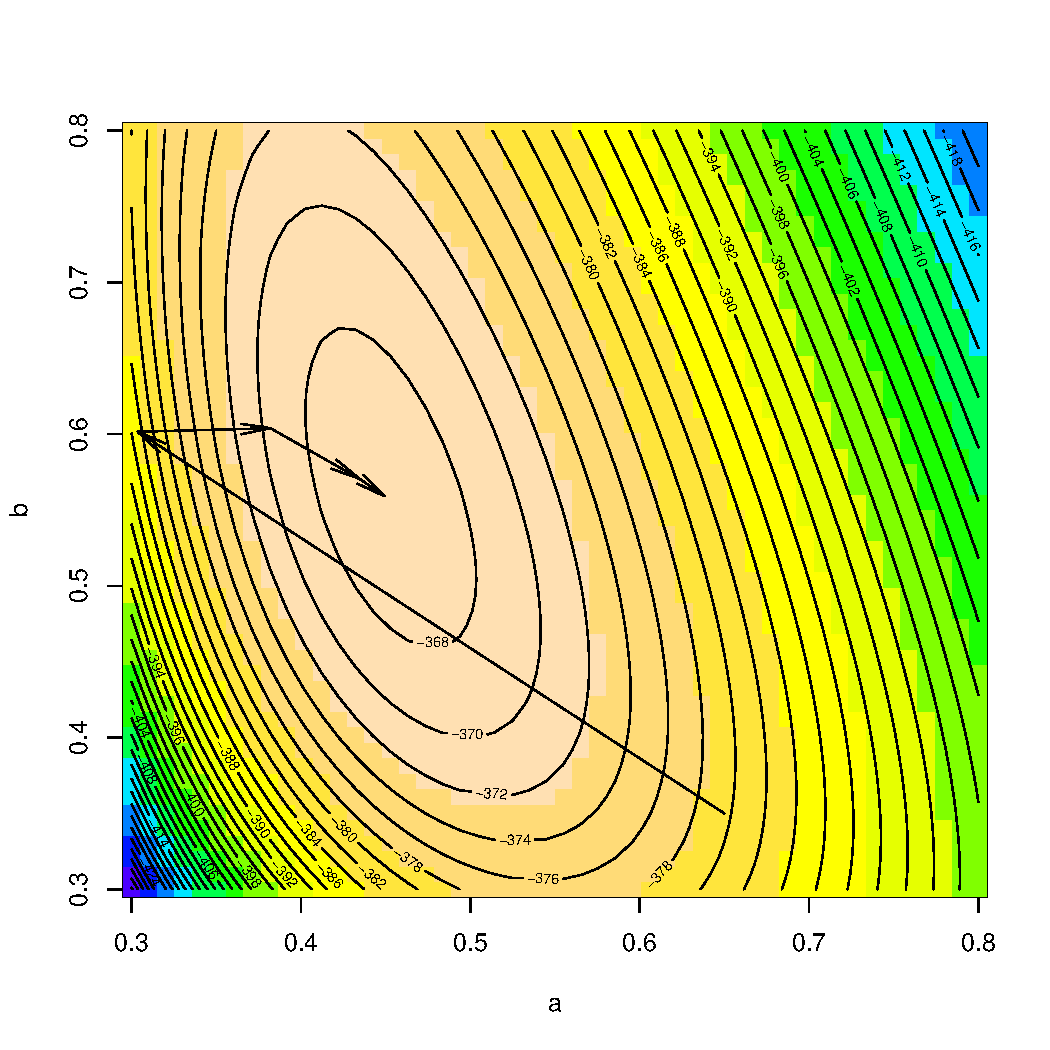
\includegraphics[trim={0em 1em 0em 3em}, clip]{nr.pdf}}
    \caption{\label{f:nr} Newton--Raphson iterates}
   \end{center}
    \end{figure}

\end{frame}

\end{document}
